
\section{Execution Model}

\subsection{Structure of SOS system}

\begin{figure}[h]
  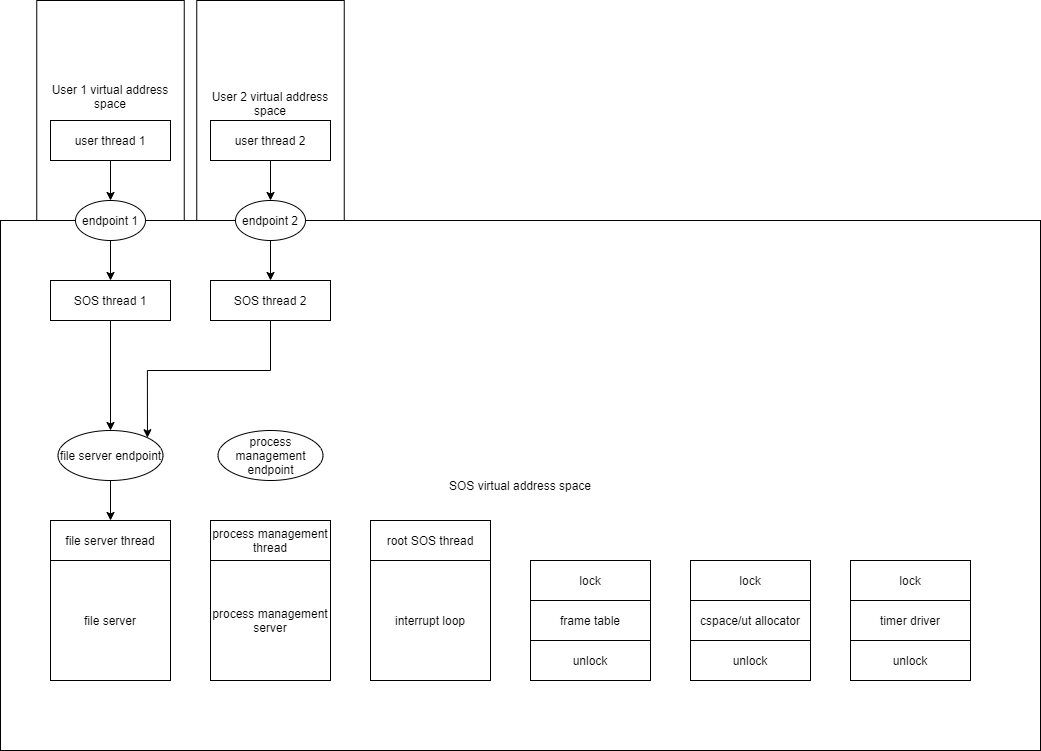
\includegraphics[width=\linewidth]{execution_model.png}
  \caption{SOS system overview}
  \label{fig:sos_overview}
\end{figure}

We use a threaded model of execution with most of the services of SOS encapsulated in servers which look like event loops. There are three main threads of execution which are spawned off from the main SOS:root thread when the system is initialized.
The main SOS:root primarily deals with the interrupt\_loop which waits on a notification object created specifically for dealing with the interrupts and once it receives a signal on that notification object it handles the IRQ corresponding to it and then 
starts waiting again for any potential interrupts. The two other main threads of control/SOS threads that exists in the system are the \textbf{File server thread} and the \textbf{Process management server}, both of them are created inside main.c.

\begin{enumerate}
  \item The file server thread when initialized starts waiting on its server loop on the specialized endpoint named file\_server\_ep for the request from the user to deal with any of the file management/updation of the 
  file interfaces already in place, it creates a new reply object to reply back to the specific user/SOS thread which has called in and then stores in the correct reply object to reply back to the user inside the call context and goes back in to the 
  server loop by creating a new reply object if it is not dealing with any interrupts/IRQs.
  \item Another major thread that we have in the system is the process management thread which is used for the global management of the user processes in the system and is again an abstraction of the SOS service broken into a separate thread of execution.
  The process management thread again waits on an ipc endpoint on which the processes can call in and it again creates a new reply object to reply back to a specific process and saves the reply object correctly inside correct index of the process management struct for the particular process 
  of which the process id is the index into the process management struct where its reply object is stored in. Whenever a new process is exec'd  a request into the process management loop is made which spawns of a new kernel thread corresponding to the new 
  user thread that is going to be created which has its own separate private endpoint to communicate back into the system and its associated SOS thread. Both the newly spawned off kernel thread/SOS thread and the user process associated with it are stored inside teh process management structure at the correct index which is new processes PID.
\end{enumerate}

\subsection{Locks for the shared objects:}

We have two types of locks in our system, and the lock objects corresponding to which are declared in the special file used for managing the  
synchronization in the system named as "\textbf{sync.h}" and the lock objects are created using the alloc\_retype and the ut\_allocator 
library provided by seL4 inside main.c, we use seL4\_wait and seL4\_Signal function calls on the lock objects to provide the 
intrinsic mechanism for the synchronization on the lock objects and the two lock objects in the system are namely corresponding to:

\begin{enumerate}
    \item Global Cspace and the ut allocator, named as \textbf{SOS\_CU\_LOCK()} which does nothing but waits on the cspace\_ut\_lock object
    implemented as seL4\_Wait(cspace\_ut\_lock, NULL) and has a corresponding \textbf{SOS\_CU\_UNLOCK()} which signals the cspace\_ut\_lock as seL4\_Signal(cspace\_ut\_lock).
    \item Lock for the Frame table accessed globally by all the processes and is created as \textbf{SOS\_FT\_LOCK()} and waits on frame\_table\_lock 
    as \textbf{SOS\_FT\_LOCK()} seL4\_Wait(frame\_table\_lock, NULL) and has a corresponding \textbf{SOS\_FT\_UNLOCK()}  which signals the frame\_table\_lock as 
    seL4\_Signal(frame\_table\_lock).
  \end{enumerate}

\noindent All other synchronization requirements in the system are dealt with implicitly by breaking and delegating the individual responsibility of to separate servers
in the system wherein each processes calls are dealt with on separate endpoint objects which makes the system implicitly synchronized and each of the server also provides an 
synchronized access to all of its management data structures Eg. process manage server provides synchronized access to process management data structures.
